\section{Scikit-Learn}
\begin{frame}
	\frametitle{Oque é?}	
	\centering
	\begin{itemize}
		\item O scikit-learn é uma biblioteca feita para simplificar o treinamento e uso de modelos de machine learning em Python
	\end{itemize}
	
\includegraphics[width=0.3\linewidth]{Scikit_learn_logo.png}
	
\includegraphics[width=0.3\linewidth]{python_logo.png}
\end{frame}
\begin{frame}
	\frametitle{Principais características}	
	\begin{itemize}
		\item Ideal para modelos de ML clássicos
		\item Ferramentas simples de pré-processamento, treino e validação
		\item API simples de usar
		\item Integração nativa com outras bibliotecas do python
	\end{itemize}
	\centering
	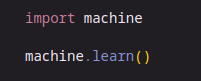
\includegraphics[width=0.25\linewidth]{eh_isso_que_eh_machine_learning?.png}
\end{frame}
\begin{frame}
	\frametitle{Oque vamos abordar}	
	\begin{itemize}
		\item Vamos ver como o tratamento e pré-processamento dos dados é uma camada importante no processo de aprendizado de máquina
		\item Vamos abordar os métodos para uso em código dos algoritmos de treino supervisionado e não supervisionado vistos
	\end{itemize}
\end{frame}